\documentclass[letterpaper,11pt]{article}

\usepackage{iftex}
\ifXeTeX
  \usepackage{fontspec}
  \setmainfont{Times New Roman}
  \usepackage{polyglossia}
  \setdefaultlanguage{vietnamese}
\else
  \usepackage[T1]{fontenc}
\fi
\usepackage[top=15mm,bottom=15mm,left=20mm,right=20mm]{geometry}
\usepackage{graphicx}
\usepackage{array,booktabs,longtable,tabularx,multirow}
\usepackage{enumitem}
\usepackage{setspace}
\usepackage[table]{xcolor}
\usepackage{titlesec}
\usepackage{caption}
\usepackage{hyperref}
\hypersetup{hidelinks}
\usepackage[backend=biber,style=numeric,sorting=nyt,maxbibnames=99]{biblatex}
\addbibresource{ref.bib}

\setlength{\parindent}{0pt}
\setlength{\parskip}{5pt}
\setstretch{1.1}
\setlist[itemize]{leftmargin=1.6em,itemsep=2pt,topsep=3pt}
\definecolor{uitblue}{RGB}{0,0,255}
\titleformat{\section}{\large\bfseries\color{uitblue}}{}{0pt}{}
\titleformat{\subsection}{\large\bfseries\color{uitblue}}{}{0pt}{}
\titleformat{\subsubsection}{\normalsize\bfseries\color{uitblue}}{}{0pt}{}
\titlespacing*{\section}{0pt}{10pt}{4pt}
\titlespacing*{\subsection}{0pt}{8pt}{3pt}
\titlespacing*{\subsubsection}{0pt}{6pt}{2pt}
\renewcommand{\arraystretch}{1.2}
\captionsetup{font=small,labelfont=it,textfont=it}

\begin{document}

\begin{tabularx}{\textwidth}{@{}X>{\raggedleft\arraybackslash}p{4.1cm}@{}}
\begin{minipage}[t]{\linewidth}\centering
\textbf{ĐẠI HỌC QUỐC GIA TP. HỒ CHÍ MINH}\par
\textbf{TRƯỜNG ĐẠI HỌC CÔNG NGHỆ THÔNG TIN}
\end{minipage} &
\begin{minipage}[t]{\linewidth}\centering
Ngày nhận hồ sơ:\par\vspace{5pt}\textit{(Do CQ quản lý ghi)}
\end{minipage}
\end{tabularx}

\begin{center}
  \vspace{14pt}
  {\Large\bfseries THUYẾT MINH\par}
  \vspace{3pt}
  {\large ĐỀ TÀI NGHIÊN CỨU KHOA HỌC SINH VIÊN 2026\par}
\end{center}

\section*{A. THÔNG TIN CHUNG}

\subsection*{A1. Tên đề tài}
\begin{itemize}[label=-]
  \item \textbf{Tên tiếng Việt (IN HOA):} BATS-AGRIGUARD: HỆ THỐNG PHÁT HIỆN VÀ CẢNH BÁO NGUY CƠ LẠM DỤNG MÃ SỐ VÙNG TRỒNG TRONG TRUY XUẤT NGUỒN GỐC CHUỖI NÔNG SẢN.
  \item \textbf{Tên tiếng Anh (IN HOA):} BATS-AGRIGUARD: A RISK-AWARE FRAMEWORK FOR DETECTING AND PREVENTING PLANTATION CODE MISUSE IN AGRICULTURAL SUPPLY CHAIN TRACEABILITY.
\end{itemize}

\subsection*{A2. Thời gian thực hiện}
6 tháng (kể từ khi được duyệt).

\subsection*{A3. Tổng kinh phí}
Tổng kinh phí: 1.000.000 đồng, gồm:
\begin{itemize}
  \item Kinh phí từ Trường Đại học Công nghệ Thông tin: 1.000.000 đồng.
\end{itemize}
\textit{Tài liệu nguồn chưa cung cấp phương án phân bổ chi tiết theo hạng mục.}

\subsection*{A4. Chủ nhiệm đề tài}
\begin{spacing}{1.15}
\hspace*{1em}Họ và tên: Nguyễn Đình Khang\par
\hspace*{1em}Ngày, tháng, năm sinh: 07/05/2005 \hfill Giới tính (Nam/Nữ): Nam\par
\hspace*{1em}Số CCCD: 080205003038; Ngày cấp: 25/04/2021; Nơi cấp: Cục trưởng Cục Cảnh sát quản lý hành chính về trật tự xã hội\par
\hspace*{1em}Mã số sinh viên: 23520694\par
\hspace*{1em}Số điện thoại liên lạc: 0967 414 607\par
\hspace*{1em}Khoa: Mạng máy tính và Truyền thông\par
\hspace*{1em}Số tài khoản: 1068762359 \hfill Ngân hàng: Vietcombank\par
\hspace*{1em}Giảng viên hướng dẫn: [Chưa có thông tin trong tài liệu nguồn]
\end{spacing}

\subsection*{A5. Thành viên đề tài (kể cả chủ nhiệm)}
\begin{center}
\begin{tabularx}{\textwidth}{|>{\centering\arraybackslash}p{0.6cm}|X|>{\centering\arraybackslash}p{2cm}|X|}
\hline
\textbf{TT} & \centering\textbf{Họ và tên} & \textbf{MSSV} & \centering\textbf{Khoa}\arraybackslash \\
\hline
1 & Nguyễn Đình Khang & 23520694 & Mạng máy tính và Truyền thông \\
\hline
2 & Võ Minh An & 23520033 & Mạng máy tính và Truyền thông \\
\hline
\end{tabularx}
\end{center}

\section*{B. MÔ TẢ NGHIÊN CỨU}

\subsection*{B1. Giới thiệu về đề tài}
Truy xuất nguồn gốc nông sản đang được nghiên cứu theo hướng kết hợp blockchain, Internet of Things và mô hình dữ liệu chuẩn hóa để tăng khả năng chia sẻ, kiểm toán và minh bạch lịch sử sản phẩm trong chuỗi cung ứng \cite{ahmad2021,ellahi2023,shahid2020,caro2018,pranto2021}. Các công trình hiện có cho thấy blockchain có thể bảo toàn lịch sử giao dịch và hỗ trợ phối hợp giữa nhiều tác nhân; những triển khai thực tế cũng đã chứng minh tiềm năng áp dụng trong chuỗi nông sản \cite{shahid2020,caro2018,spitalleri2023}.

Trong một chuỗi nông sản có nhiều tác nhân, dữ liệu vùng trồng, thu hoạch, tiếp nhận, chuyển giao, đóng gói và xuất hàng thường được hình thành ở các thời điểm và hệ thống khác nhau. Vì vậy, yêu cầu không chỉ là lưu lại các bản ghi riêng lẻ, mà còn là liên kết chúng theo một mô hình sự kiện có thể trao đổi và đối chiếu. GS1 EPCIS cung cấp cơ sở để tổ chức dữ liệu về những gì đã xảy ra với sản phẩm, thời điểm, địa điểm và tác nhân tham gia; đây là nền tảng phù hợp để đề tài xây dựng profile sự kiện truy xuất trong phạm vi PoC \cite{ahn2023}.

Tuy nhiên, một lịch sử được ghi nhận chưa mặc nhiên là lịch sử nhất quán. Một sự kiện có thể hợp lệ về cấu trúc nhưng vẫn bất thường khi đối chiếu vị trí, chủ thể, trạng thái mã vùng trồng, sản lượng hoặc quan hệ chuyển giao với các dữ liệu và sự kiện liên quan. Ví dụ, mã vùng trồng có thể được sử dụng ngoài polygon đã đăng ký; sản lượng tích lũy có thể vượt năng lực đã khai báo; đầu ra của một công đoạn có thể không tương ứng với đầu vào có nguồn gốc hợp lệ; hoặc trình tự bàn giao có thể không phù hợp với chuỗi nghiệp vụ. Dữ liệu không gian, mô hình sự kiện và các cơ chế tăng hiệu quả truy xuất là những nền tảng quan trọng, song không tự xác thực tính hợp lý của nội dung provenance \cite{ahn2023,miloudi2019,wu2023}.

Bên cạnh đó, tính bất biến của blockchain không giải quyết trực tiếp độ chính xác của dữ liệu hình thành ngoài chuỗi; một tọa độ, khối lượng hoặc bằng chứng không chính xác vẫn có thể được cam kết bất biến. Giới hạn này phù hợp với thảo luận về oracle paradox trong các hệ thống smart contract \cite{albizri2021}. Do đó, blockchain trong đề tài không được xem là cơ chế chứng minh tuyệt đối tính đúng của dữ liệu đầu vào, mà là lớp bảo toàn bằng chứng cho dữ liệu đã đi qua các bước chuẩn hóa và kiểm tra.

Từ khoảng trống giữa \textit{traceability} và \textit{provenance integrity}, đề tài BATS-AgriGuard đề xuất quy trình \textit{validation-before-anchoring}. Mỗi vùng trồng được mô hình hóa bằng \textit{Digital Plantation Identity} (DPI), liên kết mã vùng trồng với polygon địa lý, diện tích, loại cây trồng, chủ thể được ủy quyền, trạng thái và thời gian hiệu lực. Các sự kiện từ thu hoạch, tiếp nhận/chuyển giao, đóng gói đến xuất hàng được tổ chức theo hướng căn chỉnh với GS1 EPCIS. \textit{Plantation Code Integrity Engine} (PCIE) kiểm tra các ràng buộc về không gian, quyền chủ thể, trạng thái, năng lực sản lượng, bằng chứng, \textit{Mass Balance} và \textit{Chain of Custody} ở cả cấp sự kiện lẫn xuyên sự kiện.

Sau kiểm tra, dữ liệu được chuẩn hóa, băm, tổng hợp thành Merkle root và neo commitment lên blockchain EVM để hỗ trợ xác minh tính toàn vẹn sau thời điểm cam kết. Kết quả được phân loại thành \textsc{pass}, \textsc{review} hoặc \textsc{block} cùng rule kích hoạt và dữ liệu liên quan, nhằm giúp người dùng truy xuất, giải thích và hậu kiểm. Các cảnh báo của hệ thống được định vị là dấu hiệu bất thường cần xem xét, không phải kết luận tự động về hành vi gian lận.

\begin{figure}[!htbp]
  \centering
  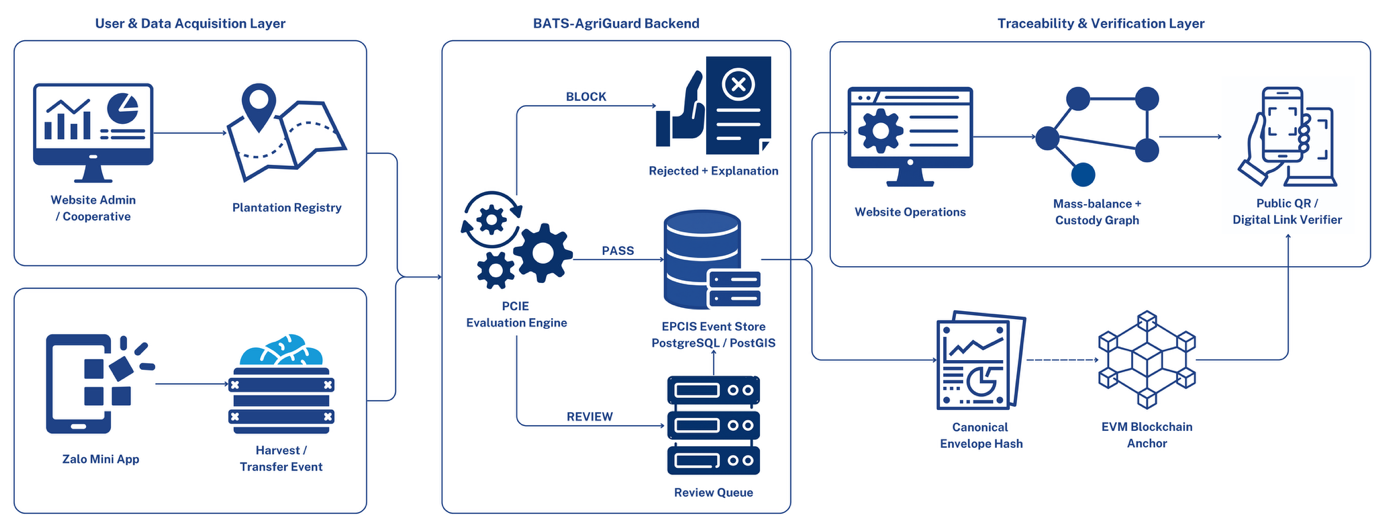
\includegraphics[width=\textwidth,height=0.35\textheight,keepaspectratio]{assets/bats-architecture.png}
  \caption{Kiến trúc tổng thể của hệ thống BATS-AgriGuard}
  \label{fig:bats-architecture}
\end{figure}

\textbf{Dựa trên hướng tiếp cận trên, đề tài dự kiến đóng góp:}
\begin{itemize}
  \item \textbf{Mô hình DPI:} biến mã số vùng trồng từ một chuỗi định danh đơn lẻ thành một thực thể số có ranh giới địa lý, diện tích, loại cây trồng, chủ thể được ủy quyền, trạng thái, thời gian hiệu lực và lịch sử sự kiện. Mô hình này tạo cơ sở để đối chiếu claim nguồn gốc với dữ liệu vùng trồng đã đăng ký.
  \item \textbf{PCIE với tám nhóm bất biến giải thích được:} \textit{Geospatial Integrity}, \textit{Identity/Authorization}, \textit{Plantation Status}, \textit{Seasonal Yield Capacity}, \textit{Evidence Duplication}, \textit{Spatio-temporal Consistency}, \textit{Mass Balance} và \textit{Chain of Custody}. PCIE mở rộng kiểm tra từ tính hợp lệ của một sự kiện sang tính nhất quán giữa nhiều sự kiện, lô hàng và chủ thể trong chuỗi.
  \item \textbf{Profile dữ liệu và luồng sự kiện căn chỉnh với GS1 EPCIS:} liên kết vùng trồng với sự kiện thu hoạch, tiếp nhận/chuyển giao, đóng gói và xuất hàng. Cách tổ chức này giúp tách rõ dữ liệu nghiệp vụ, dữ liệu không gian, bằng chứng và quan hệ custody để phục vụ trao đổi, truy vấn và hậu kiểm.
  \item \textbf{Cơ chế quyết định \textsc{pass}--\textsc{review}--\textsc{block}:} mỗi quyết định gắn với rule kích hoạt và dữ liệu liên quan. \textsc{review} được sử dụng để đưa các trường hợp cần xem xét thêm vào hàng đợi hậu kiểm, tránh đồng nhất dấu hiệu bất thường với kết luận gian lận.
  \item \textbf{Kiến trúc validation-before-anchoring:} kết hợp lớp thu thập hiện trường, PostgreSQL/PostGIS, quản lý sự kiện và bằng chứng, cùng lớp Merkle/EVM. Dữ liệu chỉ được tạo commitment sau kiểm tra; blockchain vì vậy bảo toàn tính toàn vẹn sau cam kết và hỗ trợ \textit{inclusion verification}, thay vì tự chứng minh tính đúng của dữ liệu đầu vào.
  \item \textbf{Khung kiểm chứng cho PoC:} gồm các kịch bản hợp lệ, biên và đối kháng đối với từng nhóm bất biến; đồng thời tách việc đánh giá rule engine, truy vấn không gian và Merkle để làm rõ phạm vi, giới hạn và tính khả thi kỹ thuật của từng thành phần.
\end{itemize}

\subsection*{B2. Mục tiêu, nội dung, kế hoạch nghiên cứu}
\begin{itemize}
  \item Nghiên cứu mô hình hóa dữ liệu vùng trồng, sự kiện truy xuất và các quan hệ provenance theo hướng căn chỉnh với GS1 EPCIS.
  \item Thiết kế PCIE để kiểm tra tính toàn vẹn mã số vùng trồng và tính nhất quán dữ liệu ở cấp sự kiện lẫn xuyên sự kiện.
  \item Hiện thực PoC, kiểm chứng theo các kịch bản xác định và báo cáo rõ phạm vi, giới hạn, khả năng áp dụng của hệ thống.
\end{itemize}

\subsubsection*{B2.1. Mục tiêu}
\textbf{Mục tiêu tổng quát:} Xây dựng và đánh giá BATS-AgriGuard, hệ thống truy xuất nguồn gốc nông sản dựa trên GS1 EPCIS, tập trung kiểm tra tính toàn vẹn của mã số vùng trồng và tính nhất quán nguồn gốc xuyên suốt chuỗi cung ứng.

\textbf{Mục tiêu cụ thể:}
\begin{itemize}
  \item Xây dựng mô hình DPI liên kết mã số vùng trồng với polygon địa lý, diện tích, loại cây trồng, chủ thể được ủy quyền, trạng thái và khoảng thời gian hiệu lực.
  \item Xây dựng và đánh giá PCIE với tám nhóm bất biến G/I/S/Y/D/T/M/C ở cấp sự kiện và xuyên sự kiện.
  \item Mô hình hóa các sự kiện truy xuất từ thu hoạch, chuyển giao, đóng gói đến xuất hàng theo hướng căn chỉnh với GS1 EPCIS.
  \item Xây dựng cơ chế \textsc{pass}--\textsc{review}--\textsc{block} có giải thích và cơ chế bảo toàn, xác minh bằng chứng bằng cryptographic hash, Merkle Tree và EVM blockchain anchoring.
  \item Triển khai PoC và kiểm chứng trên các kịch bản hợp lệ, biên và đối kháng.
\end{itemize}

\subsubsection*{B2.2. Nội dung và phương pháp nghiên cứu}
\subsubsection*{Nội dung 1: Khảo sát cơ sở lý thuyết và đặc tả mô hình dữ liệu}
\textbf{Mục tiêu:} Xác định cơ sở khoa học, phạm vi hệ thống, tác nhân và lược đồ dữ liệu cần thiết để mô hình hóa mã số vùng trồng cùng lịch sử provenance.

\textbf{Phương pháp thực hiện:} Nghiên cứu tài liệu về truy xuất nguồn gốc nông sản, GS1 EPCIS/CBV, dữ liệu không gian, Mass Balance, Chain of Custody và blockchain; phân tích khoảng trống giữa traceability và provenance integrity. Trên cơ sở đó, đặc tả DPI gồm mã vùng trồng, polygon, diện tích, loại cây trồng, quyền sử dụng, trạng thái và thời gian hiệu lực; mô hình hóa actor, batch, sự kiện, bằng chứng và quan hệ chuyển giao.

\textbf{Kết quả dự kiến:} Bộ đặc tả dữ liệu DPI và profile sự kiện căn chỉnh GS1 EPCIS cho chuỗi vùng trồng $\rightarrow$ thu hoạch $\rightarrow$ chuyển giao $\rightarrow$ đóng gói $\rightarrow$ xuất hàng; xác định rõ phạm vi PoC, các tác nhân và giới hạn nghiên cứu.

\subsubsection*{Nội dung 2: Xây dựng Plantation Code Integrity Engine (PCIE)}
\textbf{Mục tiêu:} Xây dựng lớp kiểm tra có thể giải thích, mở rộng đánh giá từ từng sự kiện đơn lẻ sang mối quan hệ giữa nhiều sự kiện và nhiều chủ thể.

\textbf{Phương pháp thực hiện:} Xây dựng các luật kiểm tra giải thích được ở cấp sự kiện và xuyên sự kiện. Kiểm tra cấp sự kiện gồm geofence, quyền chủ thể, trạng thái/thời hạn mã vùng trồng, năng lực sản lượng theo mùa vụ và tái sử dụng bằng chứng theo policy. Kiểm tra xuyên sự kiện gồm tính nhất quán không gian--thời gian, Mass Balance và Chain of Custody. Kết quả được tổng hợp theo cơ chế \textsc{pass}--\textsc{review}--\textsc{block}; risk score chỉ dùng để ưu tiên xem xét, không thay thế logic enforcement của các hard invariant.

\textbf{Kết quả dự kiến:} PCIE trả về quyết định, rule kích hoạt và dữ liệu liên quan phục vụ giải thích; Review Queue lưu các trường hợp cần kiểm tra bổ sung. Mỗi cảnh báo được định vị là dấu hiệu bất thường cần hậu kiểm, không phải kết luận gian lận.

\subsubsection*{Nội dung 3: Hiện thực PoC truy xuất, kiểm tra và bảo toàn bằng chứng}
\textbf{Mục tiêu:} Hiện thực một luồng vận hành tích hợp từ ghi nhận dữ liệu hiện trường đến truy xuất và xác minh bằng chứng sau kiểm tra.

\textbf{Phương pháp thực hiện:} Hiện thực lớp quản lý dữ liệu nghiệp vụ và không gian bằng PostgreSQL/PostGIS; lớp thu thập dữ liệu hiện trường trên Zalo Mini App; website quản trị, truy xuất và xác minh QR/GS1 Digital Link; backend điều phối sự kiện, validation result, evidence và audit log. Các sự kiện được kiểm tra trước khi hash, tổng hợp Merkle root và neo commitment lên mạng EVM. Bằng chứng được dùng cho inclusion verification, không thay cho cơ chế xác thực sự thật vật lý.

\textbf{Kết quả dự kiến:} Một vertical slice có thể ghi nhận dữ liệu vùng trồng và sự kiện, chạy PCIE, lưu lịch sử truy xuất, xử lý REVIEW và công bố bằng chứng Merkle/EVM sau kiểm tra. EPCIS được định vị là EPCIS-aligned trong phạm vi các ObjectEvent hỗ trợ, không tuyên bố GS1 EPCIS conformance đầy đủ.

\subsubsection*{Nội dung 4: Kiểm chứng, đánh giá và hoàn thiện báo cáo}
\textbf{Mục tiêu:} Kiểm chứng implementation theo các kịch bản xác định, đánh giá khả năng phát hiện các lớp vi phạm đã đặc tả và báo cáo rõ giới hạn của kết quả.

\textbf{Phương pháp thực hiện:} Thiết kế bộ kiểm thử độc lập gồm trường hợp hợp lệ, biên và đối kháng cho từng bất biến; dùng model-based testing cho Chain of Custody và property-based testing với seed cố định cho các tính chất của các rule. Kiểm tra profile EPCIS bằng JSON Schema chính thức trong phạm vi hỗ trợ; đánh giá metric TP, FP, TN, FN, Precision, Recall và F1 theo tập kịch bản. Thực hiện microbenchmark tách rời cho rule engine, truy vấn không gian PostGIS và Merkle; không diễn giải chúng thành latency end-to-end.

\textbf{Kết quả dự kiến:} Báo cáo kiểm chứng implementation, coverage theo từng họ bất biến, phân tích ablation và độ nhạy các tham số sản lượng/Mass Balance; báo cáo benchmark riêng cho PCIE, PostGIS và Merkle, cùng thảo luận về hạn chế và hướng phát triển.

\clearpage
\subsubsection*{B2.3. Kế hoạch nghiên cứu}
\begin{center}
\textbf{Bảng 1. Kế hoạch nghiên cứu}
\end{center}
\begin{tabularx}{\textwidth}{|>{\centering\arraybackslash}p{1.5cm}|X|X|}
\hline
\rowcolor{uitblue}\color{white}\textbf{Thời gian} & \centering\color{white}\textbf{Nội dung chính} & \centering\color{white}\textbf{Kết quả/đầu ra}\arraybackslash \\
\hline
Tháng 1 & Khảo sát tài liệu; xác định phạm vi, đối tượng, tác nhân và các khoảng trống nghiên cứu. & Khung lý thuyết, phạm vi PoC và đặc tả yêu cầu. \\
\hline
Tháng 2 & Thiết kế DPI, dữ liệu vùng trồng, profile sự kiện và các bất biến PCIE. & Đặc tả dữ liệu, rule và policy kiểm tra. \\
\hline
Tháng 3 & Hiện thực các kiểm tra cấp sự kiện; tích hợp PostgreSQL/PostGIS và quản lý evidence. & PCIE phần kiểm tra G/I/S/Y/D; dữ liệu không gian và evidence. \\
\hline
Tháng 4 & Hiện thực kiểm tra xuyên sự kiện, Mass Balance, CoC và cơ chế PASS/REVIEW/BLOCK. & PCIE phần T/M/C; Review Queue và evidence trail. \\
\hline
Tháng 5 & Tích hợp truy xuất, QR/GS1 Digital Link, Merkle commitment và EVM anchoring; xây dựng kịch bản kiểm thử. & PoC tích hợp và bộ scenario kiểm chứng. \\
\hline
Tháng 6 & Đánh giá, phân tích kết quả, hoàn thiện báo cáo và sản phẩm trình bày. & Báo cáo tổng kết, kết quả kiểm chứng và đề xuất hướng phát triển. \\
\hline
\end{tabularx}

\subsection*{B3. Kết quả dự kiến}
\begin{itemize}
  \item Mô hình DPI cho mã số vùng trồng, liên kết dữ liệu không gian, chủ thể, trạng thái, thời hạn hiệu lực và lịch sử sự kiện.
  \item PCIE thực thi tám nhóm bất biến G/I/S/Y/D/T/M/C ở cấp sự kiện và xuyên sự kiện, có giải thích cho kết quả \textsc{pass}, \textsc{review} hoặc \textsc{block}.
  \item PoC BATS-AgriGuard gồm lớp thu thập dữ liệu hiện trường, website quản trị/truy xuất, backend, PostgreSQL/PostGIS, EPCIS Event Store, Review Queue, QR/GS1 Digital Link và lớp Merkle/EVM anchoring.
  \item Bộ kiểm thử mô tả rõ kịch bản hợp lệ, biên và đối kháng; báo cáo kiểm chứng implementation, metric phân loại, ablation, phân tích độ nhạy và microbenchmark theo từng thành phần.
  \item Báo cáo khoa học làm rõ đóng góp validation-before-anchoring, giới hạn của dữ liệu synthetic, giới hạn của blockchain đối với dữ liệu đầu vào, và các hạng mục cần hardening/pilot thực địa.
\end{itemize}
\textit{Giới hạn cần nêu trong báo cáo: Hệ thống kiểm tra tính nhất quán của dữ liệu được cung cấp, không xác nhận chất lượng hoặc an toàn thực phẩm, không thay thế cơ quan quản lý/tổ chức chứng nhận/kiểm tra thực địa, và không coi bất thường là bằng chứng trực tiếp của hành vi gian lận.}

\printbibliography[title={B4. Tài liệu tham khảo}]

\vfill
\begin{tabularx}{\textwidth}{XX}
\centering Ngày \ldots\ldots\ tháng \ldots\ldots\ năm 2026\par
\textbf{GIẢNG VIÊN HƯỚNG DẪN}\par
(Ký và ghi rõ họ tên) &
\centering Ngày \ldots\ldots\ tháng \ldots\ldots\ năm 2026\par
\textbf{CHỦ NHIỆM ĐỀ TÀI}\par
(Ký và ghi rõ họ tên)\par\vspace{3.4cm}\textbf{Nguyễn Đình Khang}
\end{tabularx}

\end{document}
